\documentclass[aspectratio=169]{beamer}
\usetheme{Madrid}
\usecolortheme{seahorse}
\usepackage{booktabs}
\usepackage{graphicx}
\usepackage{amsmath}
\usepackage{tikz}

\graphicspath{{./}}

\title{PEM Fuel Cell Stack --- Experimental Results}
\subtitle{TR-Current Experiments: 3.3\,\(\Omega\) and 6.8\,\(\Omega\) loads}
\author[LAGHA Khalil]{%
    \textbf{LAGHA Khalil}\\[0.3em]
    {\small Supervisor: Emmanuel Witrant}
}
\institute[GIPSA-lab / UGA]{%
    GIPSA-lab --- Universit\'{e} Grenoble Alpes
}
\date{June 2026}

\begin{document}

%% ── Title ───────────────────────────────────────────────────────────────────
\begin{frame}
    \begin{tikzpicture}[remember picture, overlay]
        \node[anchor=north west, inner sep=8pt] at (current page.north west)
            {
\includegraphics[height=1.1cm]{UGAlogo.png}};
        \node[anchor=north east, inner sep=8pt] at (current page.north east)
            {
\includegraphics[height=1.1cm]{gipsa-lablogo.jpg}};
    \end{tikzpicture}
    \titlepage
\end{frame}

%% ── Outline ─────────────────────────────────────────────────────────────────
\begin{frame}{Outline}
    \tableofcontents
\end{frame}

%%%%%%%%%%%%%%%%%%%%%%%%%%%%%%%%%%%%%%%%%%%%%%%%%%%%%%%%%%%%%%%%%%%%%%%%%%%
\section{Experimental Data}
%%%%%%%%%%%%%%%%%%%%%%%%%%%%%%%%%%%%%%%%%%%%%%%%%%%%%%%%%%%%%%%%%%%%%%%%%%%

\begin{frame}{Experiment 1 --- 3.3\,\(\Omega\) Load}
    \begin{columns}[c]
        \column{0.62\textwidth}
        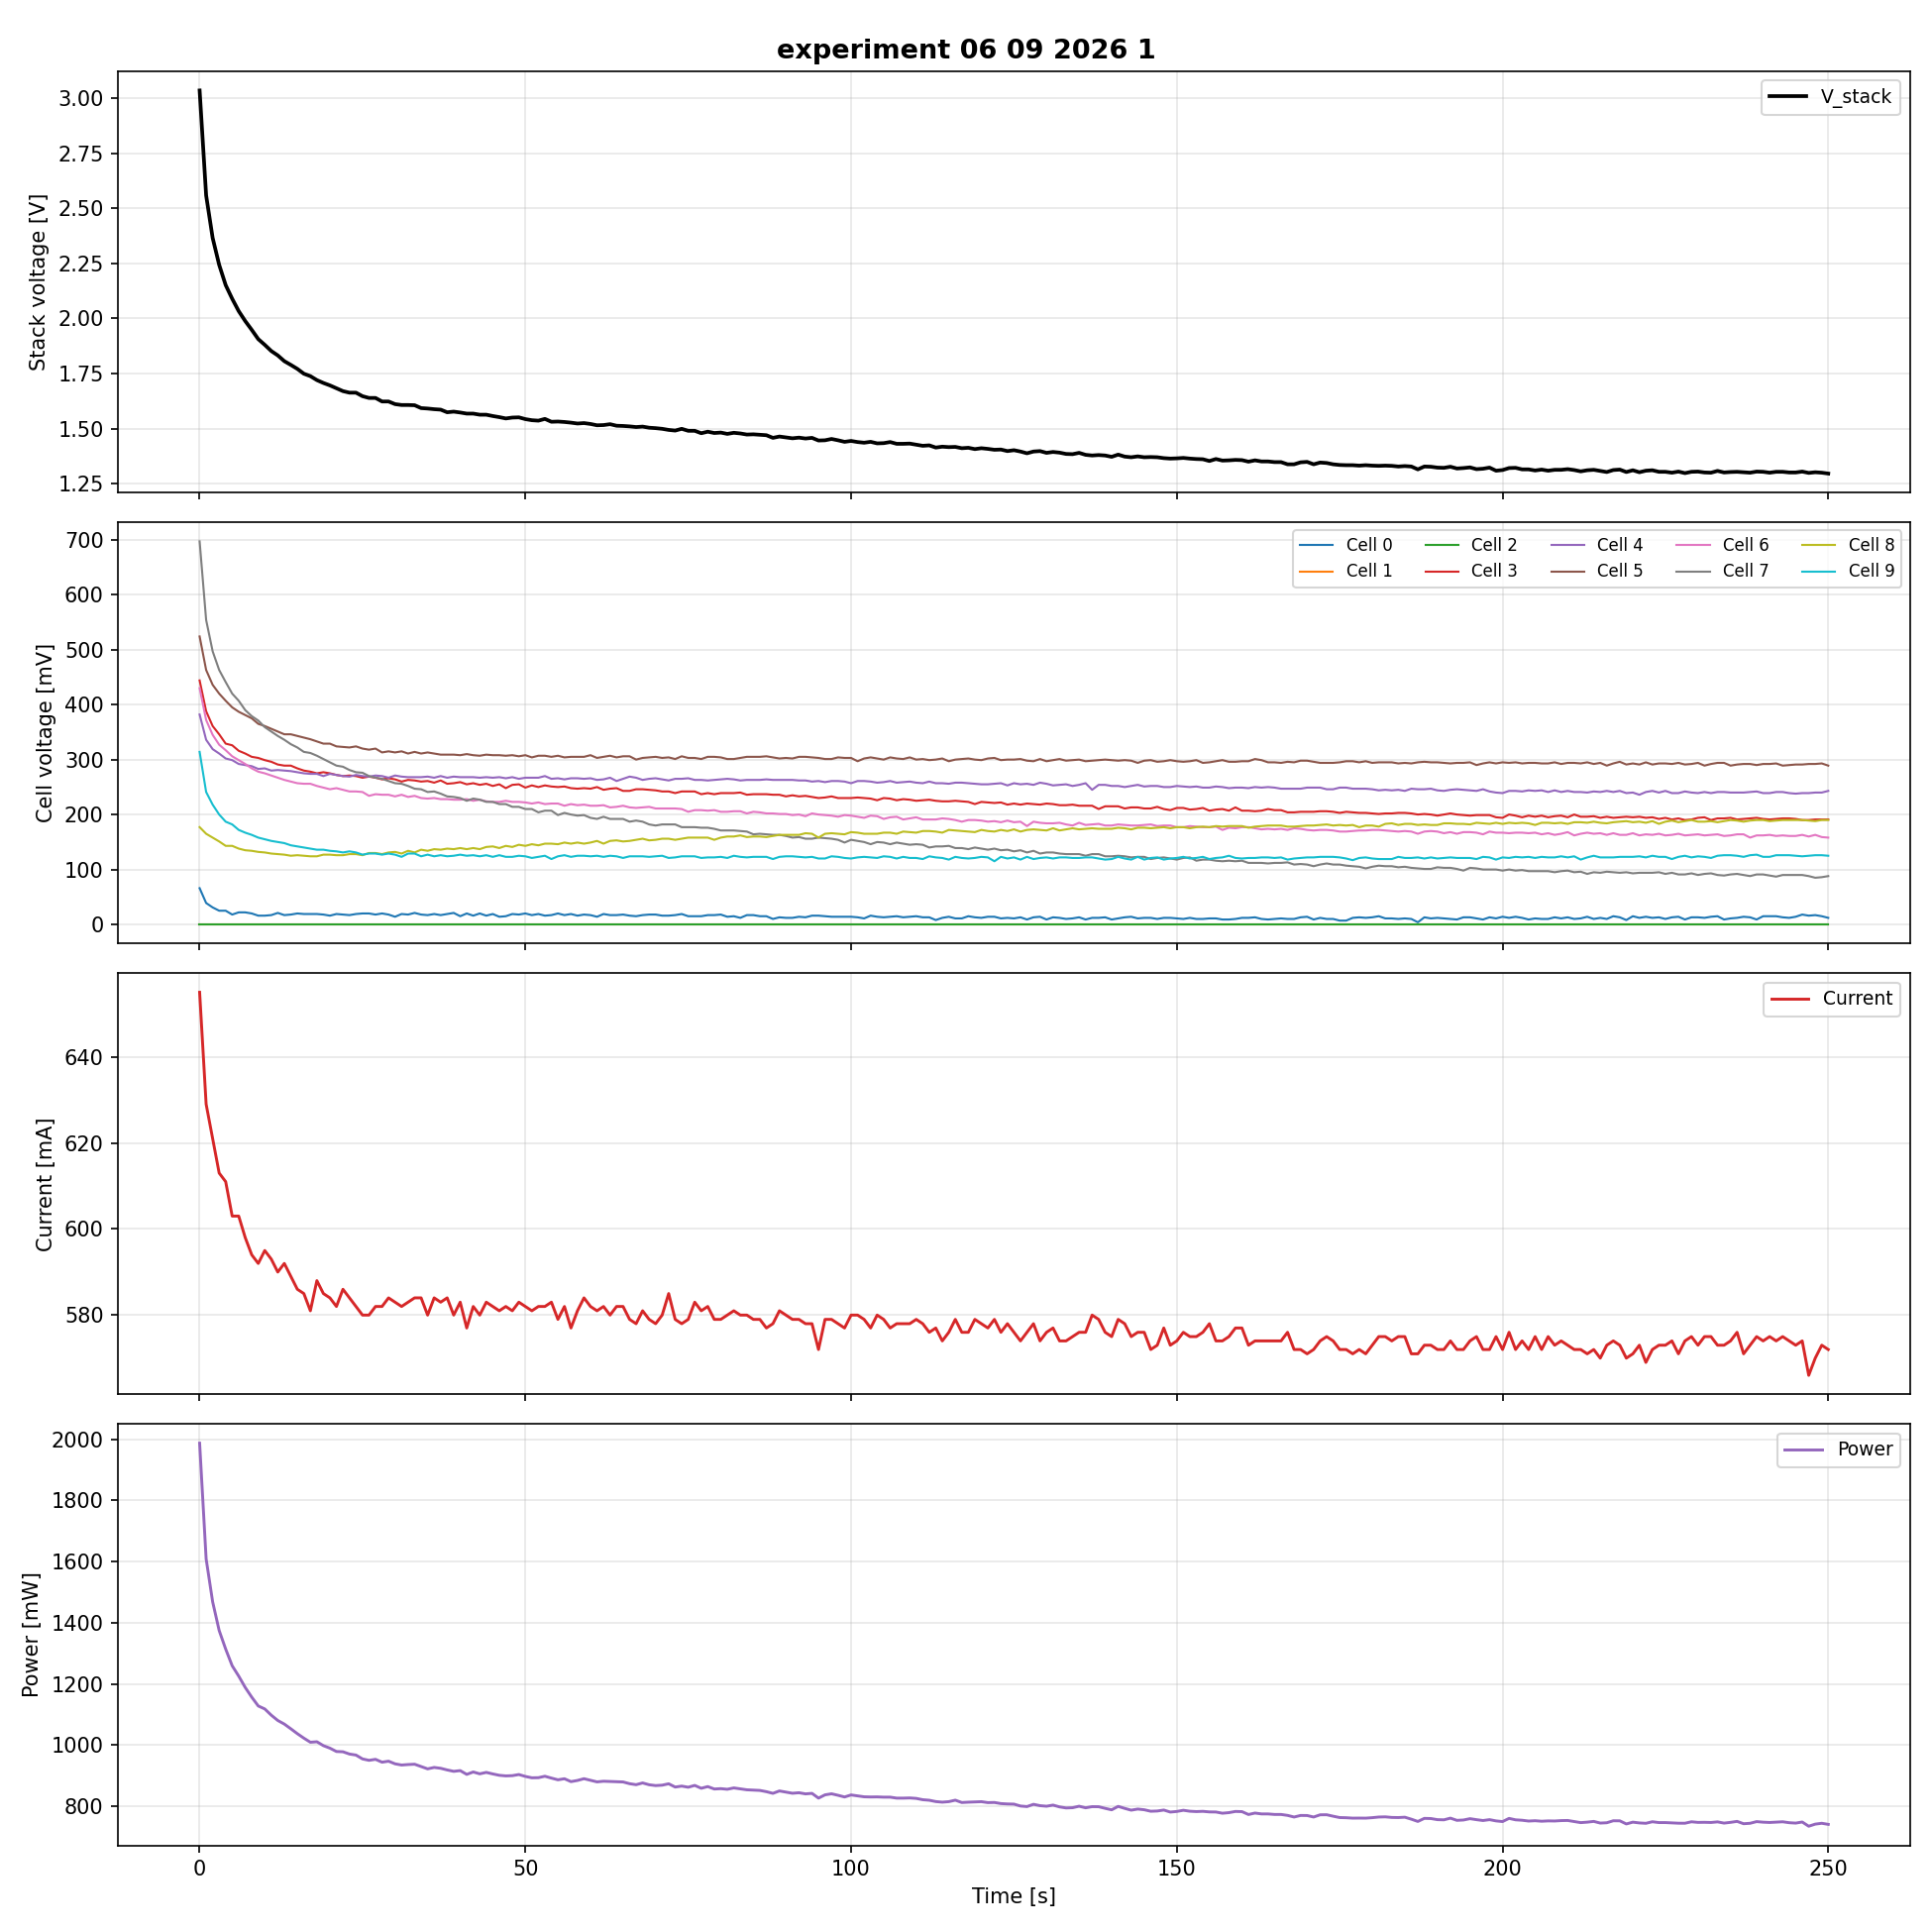
\includegraphics[height=0.82\textheight,keepaspectratio]{exp1_plot.png}
        \column{0.35\textwidth}
        \small
        \textbf{Conditions}\\[0.4em]
        $R = 3.3\,\Omega$, recorded 9 June 2026\\[0.6em]
        \textbf{Channels (top to bottom)}\\[0.3em]
        \begin{enumerate}
            \item Stack voltage $V_{\text{stack}}$ [V]
            \item Cell voltages $v_0\ldots v_9$ [mV]
            \item Current $I$ [mA]
            \item Power $P = V_{\text{stack}}\cdot I$ [mW]
        \end{enumerate}
        \vspace{0.5em}
        {\footnotesize Cells 1 \& 2 read $\approx 0\,$mV --- hardware issue.}
    \end{columns}
\end{frame}

\begin{frame}{Experiment 4 --- 6.8\,\(\Omega\) Load}
    \begin{columns}[c]
        \column{0.62\textwidth}
        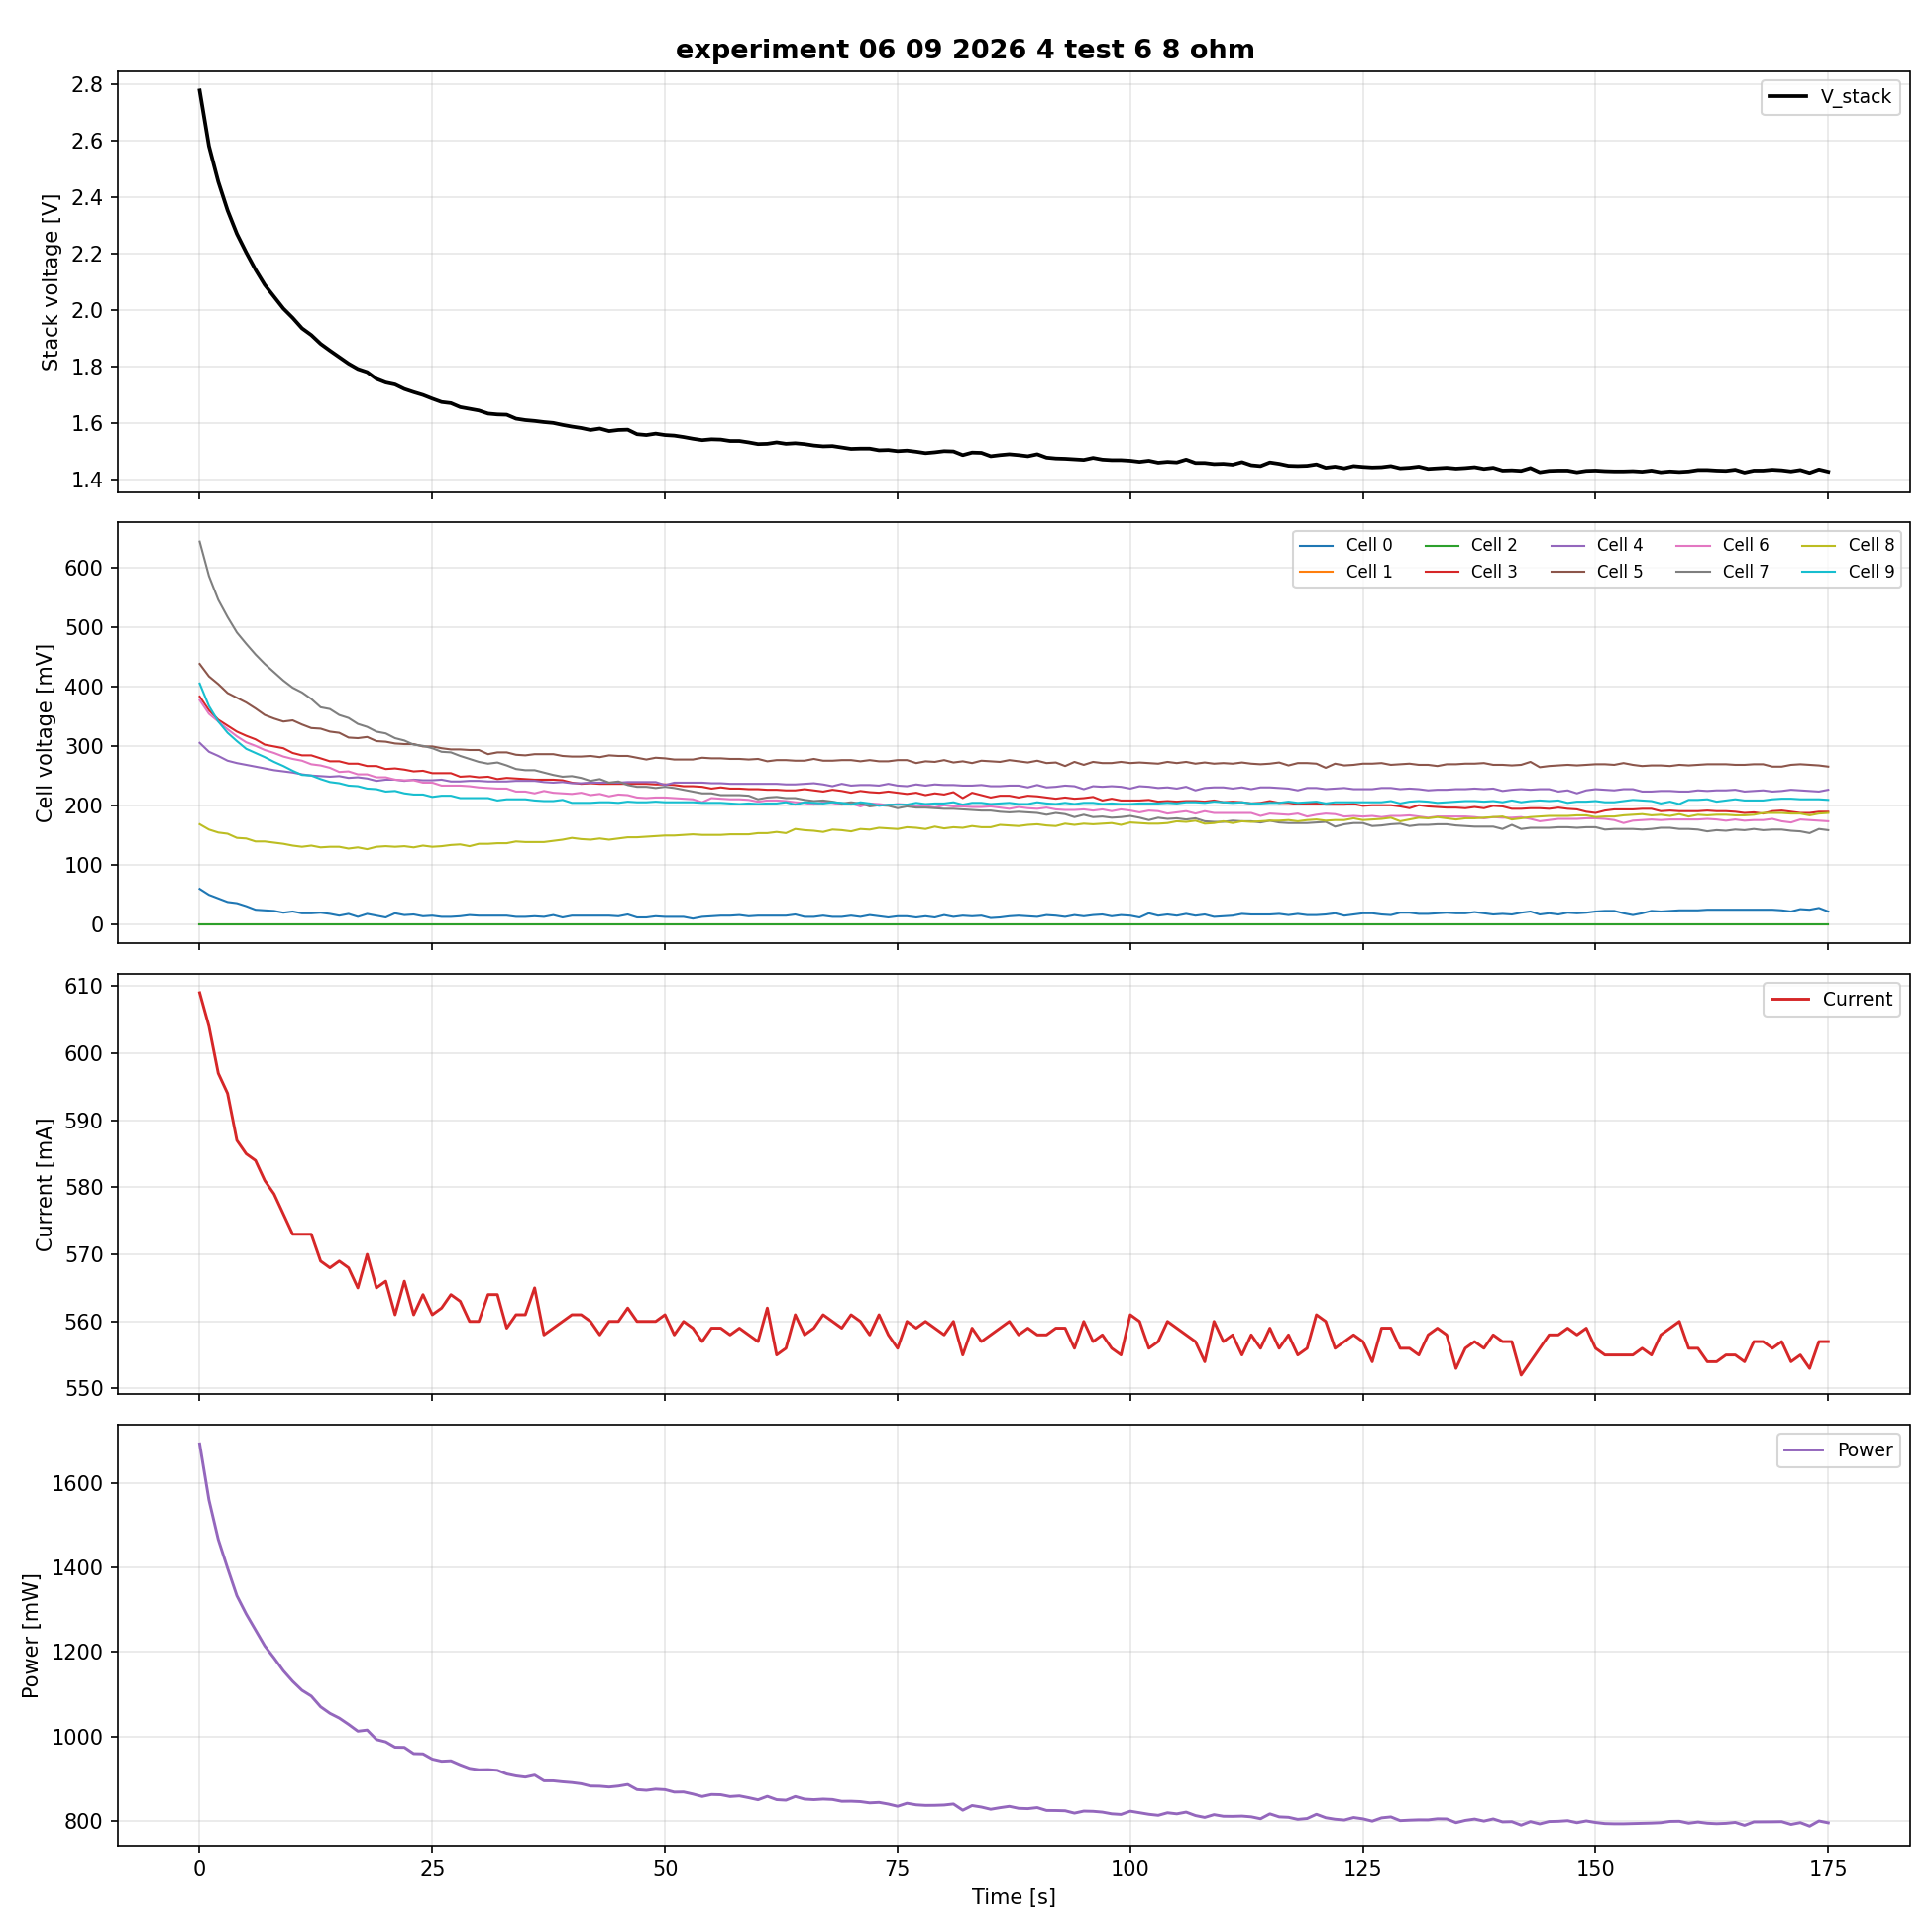
\includegraphics[height=0.82\textheight,keepaspectratio]{exp4_plot.png}
        \column{0.35\textwidth}
        \small
        \textbf{Conditions}\\[0.4em]
        $R = 6.8\,\Omega$, recorded 9 June 2026\\[0.6em]
        \textbf{Channels (top to bottom)}\\[0.3em]
        \begin{enumerate}
            \item Stack voltage $V_{\text{stack}}$ [V]
            \item Cell voltages $v_0\ldots v_9$ [mV]
            \item Current $I$ [mA]
            \item Power $P = V_{\text{stack}}\cdot I$ [mW]
        \end{enumerate}
        \vspace{0.5em}
        {\footnotesize Data starts at the current peak.\\Same dead cells observed.}
    \end{columns}
\end{frame}

%%%%%%%%%%%%%%%%%%%%%%%%%%%%%%%%%%%%%%%%%%%%%%%%%%%%%%%%%%%%%%%%%%%%%%%%%%%
\section{Current Response Time Analysis}
%%%%%%%%%%%%%%%%%%%%%%%%%%%%%%%%%%%%%%%%%%%%%%%%%%%%%%%%%%%%%%%%%%%%%%%%%%%

\begin{frame}{Current Response --- Exponential Decay Model}
    After resistor connection the current follows a decaying step:
    \[
        I(t) \;=\; I_{\text{ss}} + \Delta I \cdot e^{-t/\tau}
    \]
    \begin{itemize}
        \item \(I_{\text{ss}}\): steady-state current (mean of last 20\,\% of samples)
        \item \(\Delta I = I(0) - I_{\text{ss}}\): step amplitude
        \item \(\tau\): time constant (least-squares exponential fit)
    \end{itemize}
    \medskip
    Settling times derived analytically from the fit:
    \[
        T_{s,5\%} = -\tau\ln(0.05), \qquad T_{s,2\%} = -\tau\ln(0.02)
    \]
    Fall time 90\,\%\,\(\to\)\,10\,\% from the measured signal directly.
\end{frame}

\begin{frame}{Response Time Results}
    \begin{center}
        
\includegraphics[width=0.90\linewidth]{response_time_plot.png}
    \end{center}
\end{frame}

\begin{frame}{Response Time Metrics --- Current Summary}
    \begin{center}
    \begin{tabular}{lcc}
        \toprule
        \textbf{Metric} & \textbf{3.3\,\(\Omega\)} & \textbf{6.8\,\(\Omega\)} \\
        \midrule
        Steady-state current \(I_{\text{ss}}\) [mA] & 572.9 & 556.1 \\
        Step amplitude \(\Delta I\) [mA]             &  82.1 &  52.9 \\
        Time constant \(\tau\) [s]                   &   8.2 &  10.3 \\
        Settling time \(T_{s,5\%}\) [s]              &  24.5 &  30.8 \\
        Settling time \(T_{s,2\%}\) [s]              &  32.0 &  40.2 \\
        Fall time 90\,\%\,\(\to\)\,10\,\% [s]        &  16.0 &  19.0 \\
        \bottomrule
    \end{tabular}
    \end{center}
    \vspace{0.5em}
    \begin{block}{Observation}
        The 6.8\,\(\Omega\) load draws less current (\(\approx25\,\%\) smaller
        \(\Delta I\)) and responds \(\approx 25\,\%\) slower
        (\(\tau = 10.3\,\)s vs.\,8.2\,s), consistent with lower electrochemical
        activity at reduced current.
    \end{block}
\end{frame}

%%%%%%%%%%%%%%%%%%%%%%%%%%%%%%%%%%%%%%%%%%%%%%%%%%%%%%%%%%%%%%%%%%%%%%%%%%%
\section{Voltage Response Time Analysis}
%%%%%%%%%%%%%%%%%%%%%%%%%%%%%%%%%%%%%%%%%%%%%%%%%%%%%%%%%%%%%%%%%%%%%%%%%%%

\begin{frame}{Voltage Response --- Exponential Decay Model}
    After resistor connection the stack voltage also follows a decaying step:
    \[
        V(t) \;=\; V_{\text{ss}} + \Delta V \cdot e^{-t/\tau_V}
    \]
    \begin{itemize}
        \item \(V_{\text{ss}}\): steady-state stack voltage
        \item \(\Delta V = V(0) - V_{\text{ss}}\): voltage drop amplitude
        \item \(\tau_V\): voltage time constant (independent fit from current)
    \end{itemize}
    \medskip
    The voltage time constant is generally larger than the current time constant
    because the membrane hydration and gas pressures relax on a slower timescale.
\end{frame}

\begin{frame}{Voltage Response Time Results}
    \begin{center}
        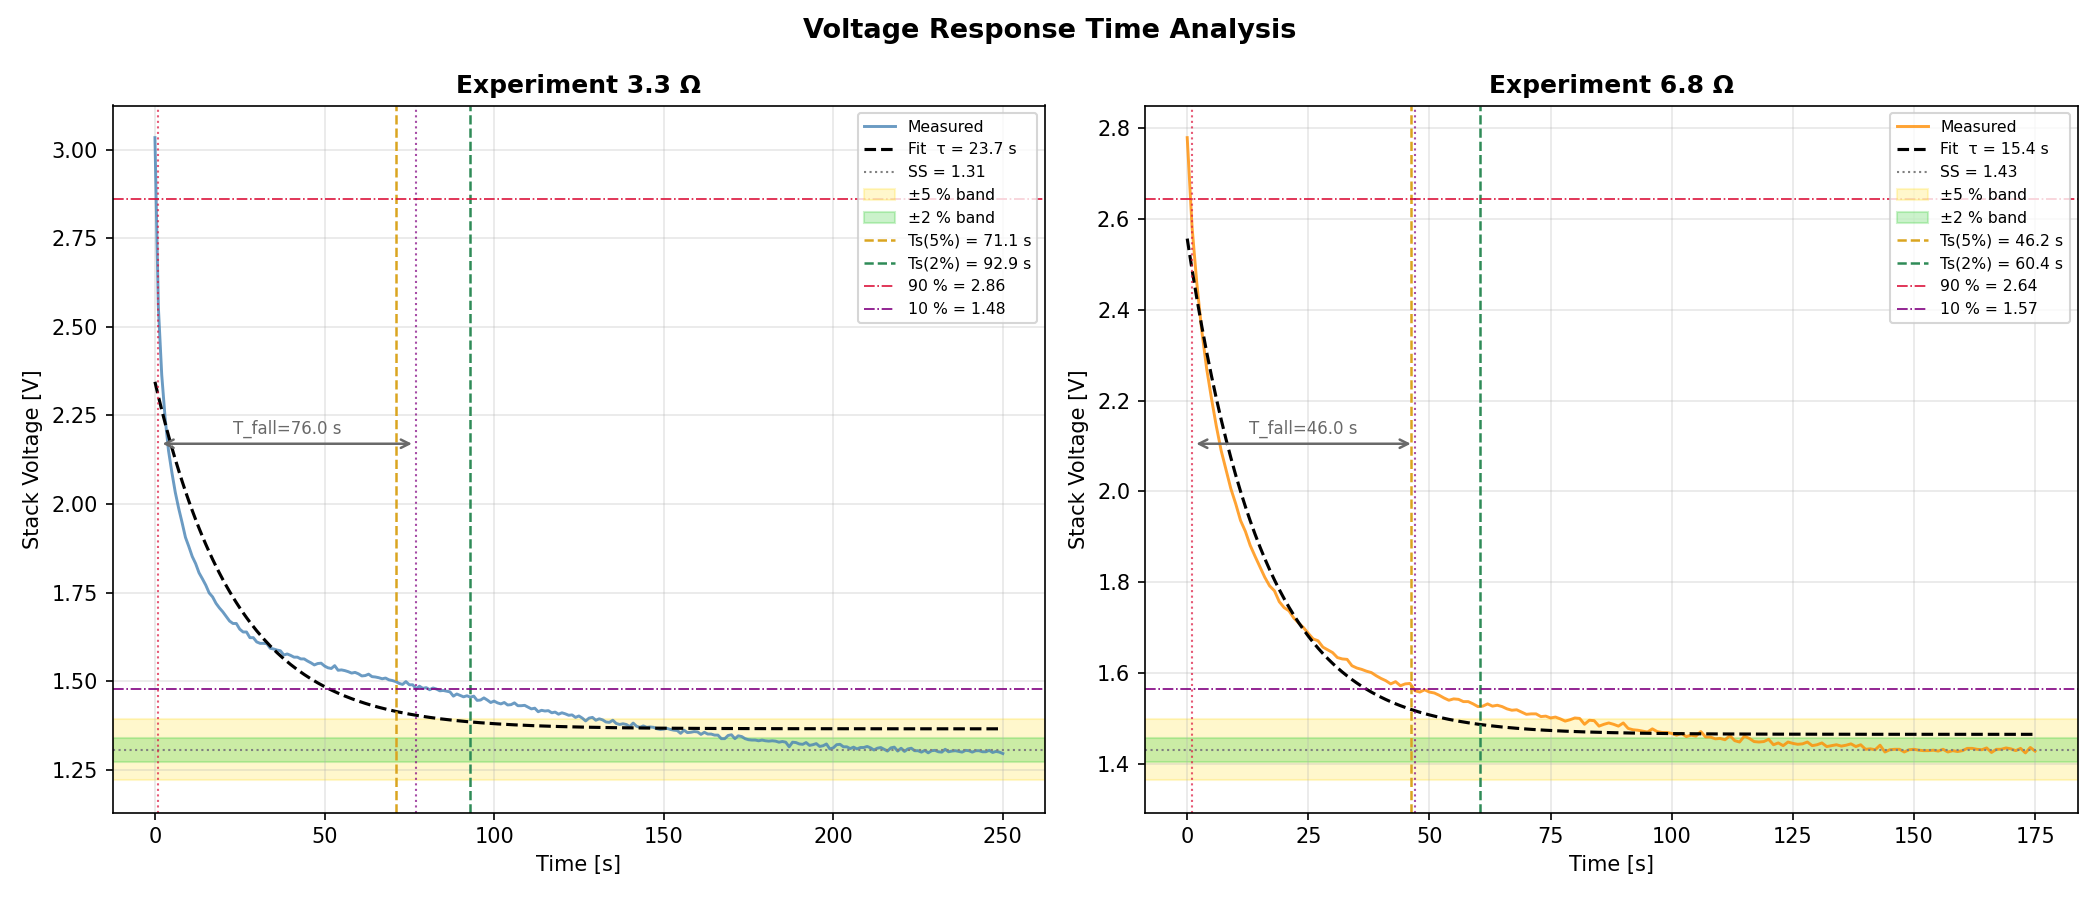
\includegraphics[width=0.90\linewidth]{voltage_response_time_plot.png}
    \end{center}
\end{frame}

\begin{frame}{Response Time Metrics --- Voltage Summary}
    \begin{center}
    \begin{tabular}{lcc}
        \toprule
        \textbf{Metric} & \textbf{3.3\,\(\Omega\)} & \textbf{6.8\,\(\Omega\)} \\
        \midrule
        Steady-state voltage \(V_{\text{ss}}\) [V]   & 1.307 & 1.431 \\
        Step amplitude \(\Delta V\) [V]              & 1.728 & 1.348 \\
        Time constant \(\tau_V\) [s]                 &  23.7 &  15.4 \\
        Settling time \(T_{s,5\%}\) [s]             &  71.2 &  46.3 \\
        Settling time \(T_{s,2\%}\) [s]             &  92.9 &  60.4 \\
        Fall time 90\,\%\,\(\to\)\,10\,\% [s]       &  76.0 &  46.0 \\
        \bottomrule
    \end{tabular}
    \end{center}
    \vspace{0.5em}
    \begin{block}{Observation}
        The 3.3\,\(\Omega\) load produces a larger voltage drop (\(\Delta V = 1.73\,\)V)
        and a slower voltage response (\(\tau_V = 23.7\,\)s vs.\,15.4\,s),
        while the current settles faster. This indicates that membrane and
        gas-management dynamics dominate the voltage relaxation.
    \end{block}
\end{frame}

%%%%%%%%%%%%%%%%%%%%%%%%%%%%%%%%%%%%%%%%%%%%%%%%%%%%%%%%%%%%%%%%%%%%%%%%%%%
\section{Conclusions}
%%%%%%%%%%%%%%%%%%%%%%%%%%%%%%%%%%%%%%%%%%%%%%%%%%%%%%%%%%%%%%%%%%%%%%%%%%%

\begin{frame}{Conclusions}
    \begin{enumerate}
        \item \textbf{Data acquisition and preprocessing}\\
              Automatic resistor-connection detection and time trimming pipeline
              implemented in Python.  Two clean datasets produced.

        \item \textbf{Current response}\\
              Exponential decay fits: $\tau_I = 8.2\,$s (3.3\,$\Omega$) and
              $\tau_I = 10.3\,$s (6.8\,$\Omega$). Current settling time $T_{s,2\%}$:
              32\,s and 40\,s respectively.

        \item \textbf{Voltage response}\\
              Voltage relaxes more slowly: $\tau_V = 23.7\,$s (3.3\,$\Omega$) and
              $\tau_V = 15.4\,$s (6.8\,$\Omega$). Settling time $T_{s,2\%}$:
              93\,s and 60\,s. The membrane and gas-management dynamics
              dominate voltage relaxation.
    \end{enumerate}
    \vspace{0.5em}
    \textbf{Next steps:} Use the measured step responses to characterise
    stack dynamics and design a closed-loop controller.
\end{frame}

%% ── Thank you ────────────────────────────────────────────────────────────────
\begin{frame}
    \begin{center}
        \Huge\textbf{Thank you}\\[1em]
        \Large Questions?
    \end{center}
\end{frame}

\end{document}
